\section{User Interface}\label{sec:results}
The goal of this project was to provide a simple way for developers to reduce information overload. It was very important that the user interface of the Chrome extension was as simple as possible to remove any possible hurdles. Figure \ref{fig:chromeExtensionInterfaceScreenshot} shows the user interface for the popup component of the Chrome extension. 

\begin{figure}[H]
\centering
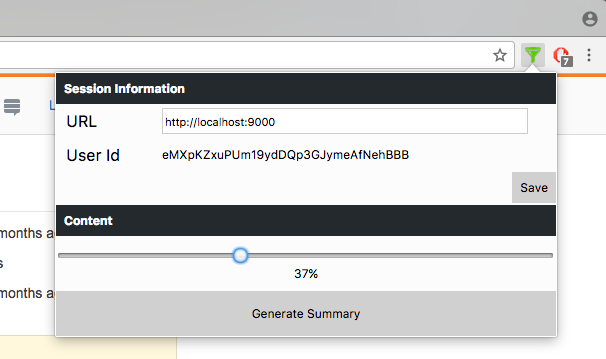
\includegraphics{Figures/ChromeUI}
\caption{Interface of the Chrome extension}
\label{fig:chromeExtensionInterfaceScreenshot}
\end{figure}

The interface consists of two main sections. The first section shows information about the current session. This was mostly used while debugging the application. The second section is used to interact with the user. The current view shows the slider, which means that the data gathering and ranking processes have completed successfully. In case of errors, or while the content script is parsing the page, the slider is hidden and messages are shown to inform the user of the current status. 

An additional visual feedback is provided by the possible icons of the extension shown in Figure \ref{fig:icons}, which can represent any of the following states:
\begin{itemize}
\item \textbf{Inactive}\\
Represented by a greyed out icon (Figure \ref{fig:chromeInactive}), tells the user that the extension is not active in the current website.
\item \textbf{Parsing}\\
While the application is parsing, a yellow icon (Figure \ref{fig:chromeParsing}) is shown to indicate that the Chrome extension is working, and the results will be shown shortly.
\item \textbf{Ready}\\
When the icon turns green (Figure \ref{fig:chromeReady}), the user has the ability to open the popup and start manipulating the content by dragging the slider.
\item \textbf{Error}\\
If an error occurs, a red icon is shown (Figure \ref{fig:chromeError}). 
\end{itemize}
\newcommand{\figureScale}{0.25}
\newcommand{\innerScale}{0.15}


\begin{figure}[H]
\centering
\begin{subfigure}[b]{\figureScale\textwidth}
\centering
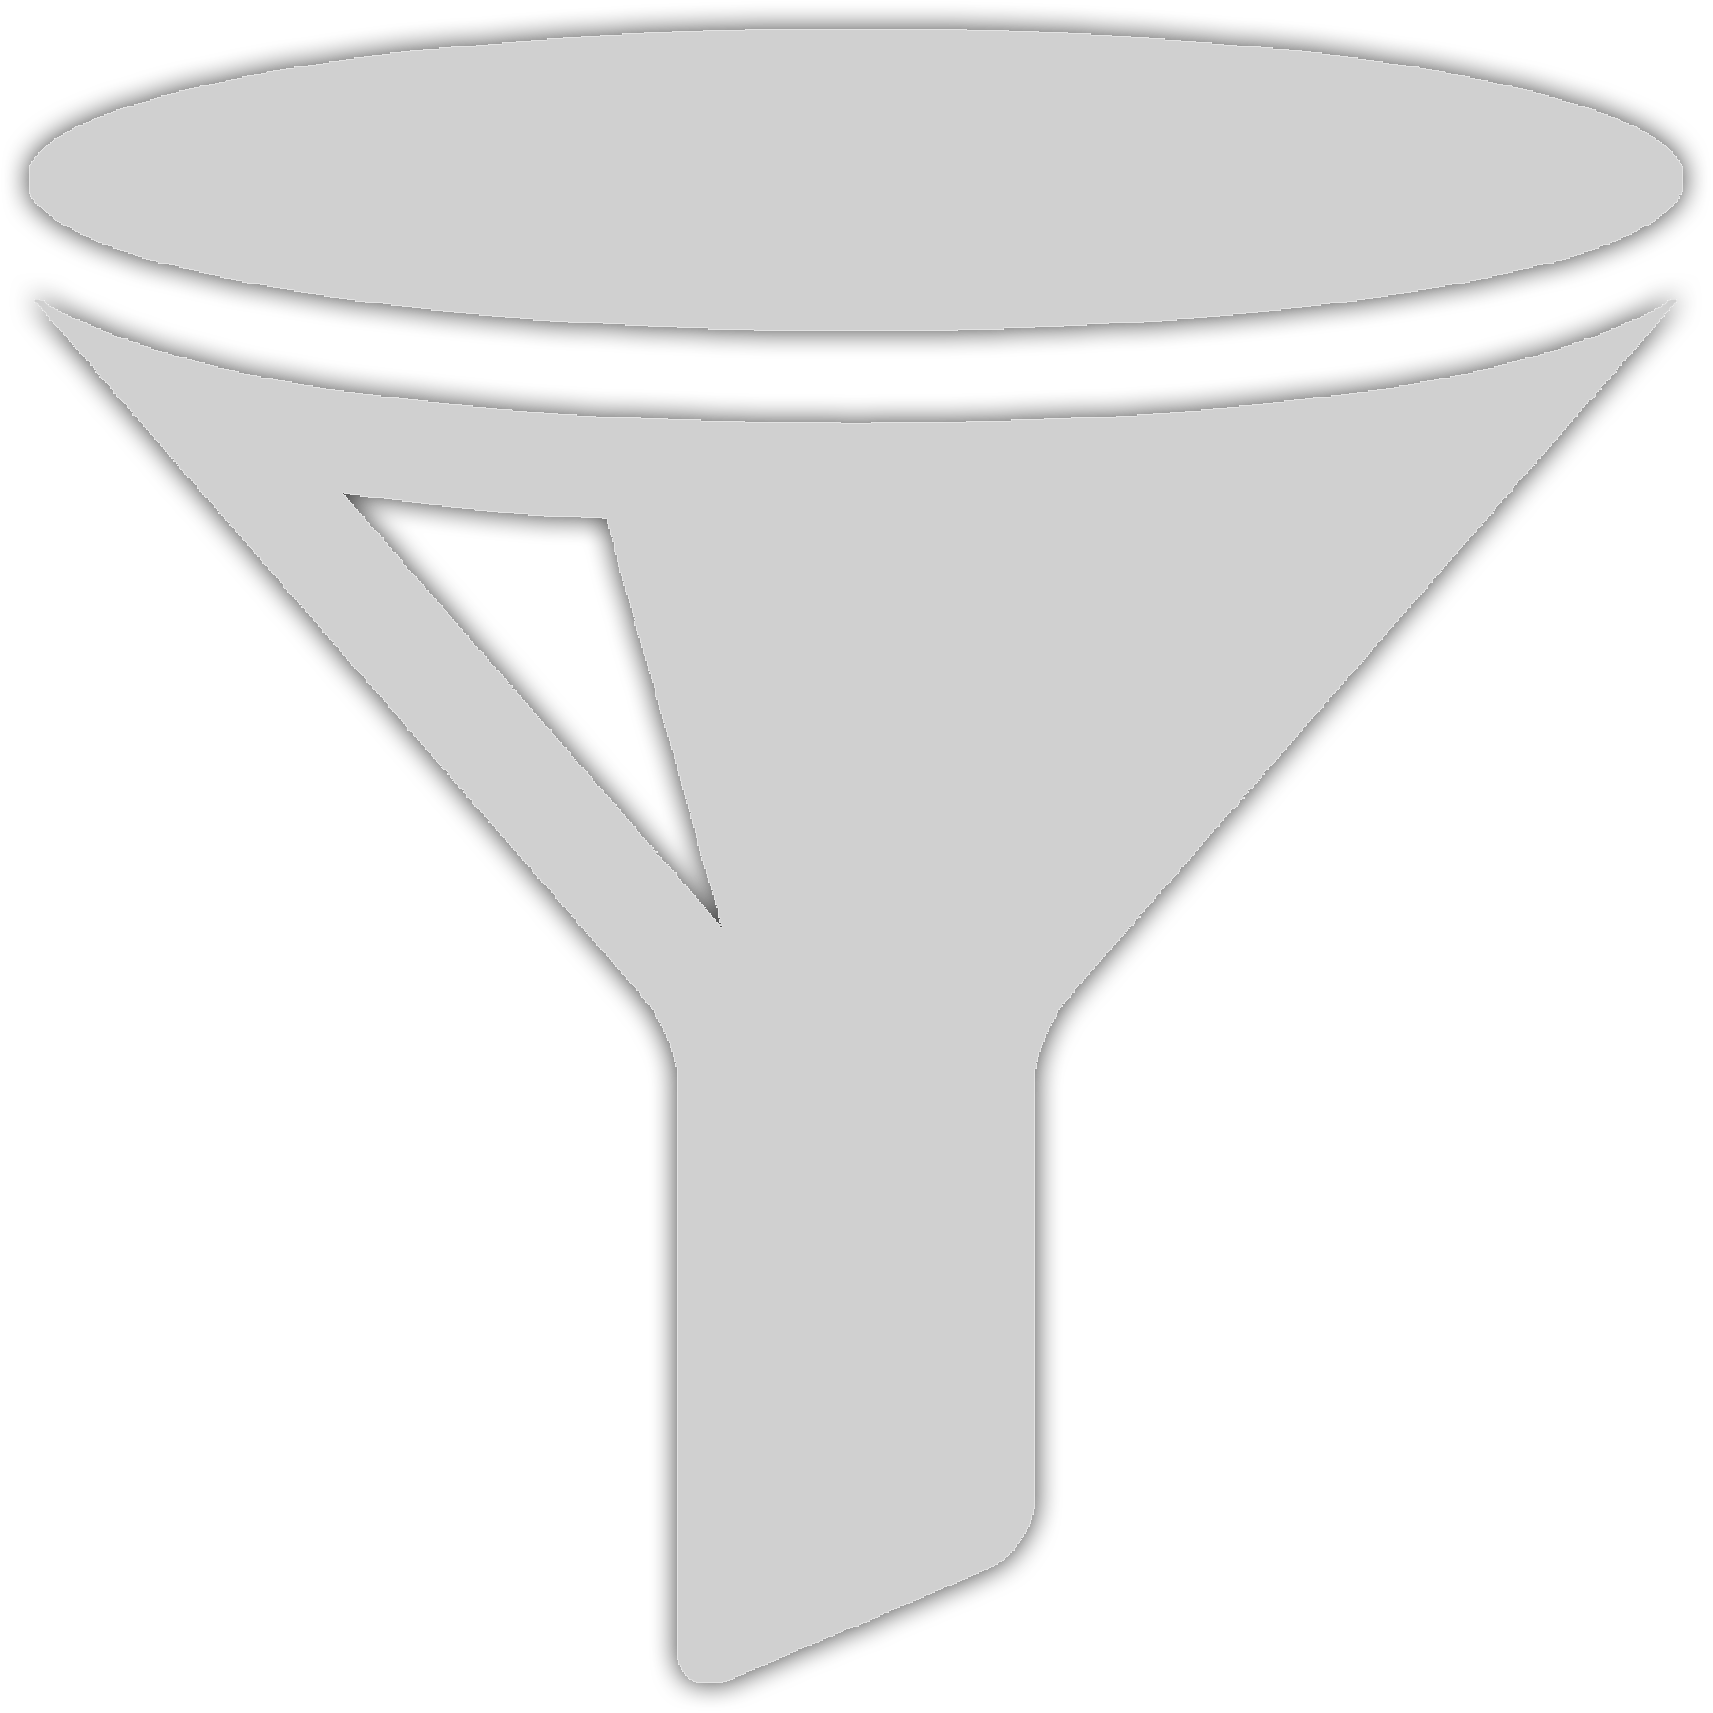
\includegraphics[scale=\innerScale]{Figures/greyPlain}
\caption{Inactive}
\label{fig:chromeInactive}
\end{subfigure}~
\begin{subfigure}[b]{\figureScale\textwidth}
\centering

\includegraphics[scale=\innerScale]{Figures/yellowPlain}
\caption{Parsing}
\label{fig:chromeParsing}
\end{subfigure}~
\begin{subfigure}[b]{\figureScale\textwidth}
\centering

\includegraphics[scale=\innerScale]{Figures/greenPlain}
\caption{Ready}
\label{fig:chromeReady}
\end{subfigure}~
\begin{subfigure}[b]{\figureScale\textwidth}
\centering

\includegraphics[scale=\innerScale]{Figures/redPlain}
\caption{Error}
\label{fig:chromeError}
\end{subfigure}
\caption{Chrome extension status icons}\label{fig:icons}
\end{figure}

When the Chrome extension has received the data back from the web service, the icon turns green and the slider is shown in the popup. The user has now the ability to choose the amount of filtration required, which updates the content of the page in real time. Any time the slider is dragged, the popup will fire an event caught by the content script, which will take care of hiding or showing the different units, depending on their sort order.


Another feature of \projectName~is the ability to generate an overview of all the pages in a user's history. By clicking the ``Generate Summary'' button from the popup (Figure \ref{fig:chromeExtensionInterfaceScreenshot}), the extension will open a new page, containing the documents. An example is shown in Figure \ref{fig:chromeExtensionSummaryScreenshot}.

For each page, a slider is available to once again filter the content independently from the other pages. An additional slider is added at the top of the page, called a master slider, which controls the amount of information displayed by each site, regardless of the value chosen by each individual slider. This allows the user to consult only the highest ranked units in its history, giving a very quick overview of multiple sites at the same time.
\begin{figure}[H]
\centering
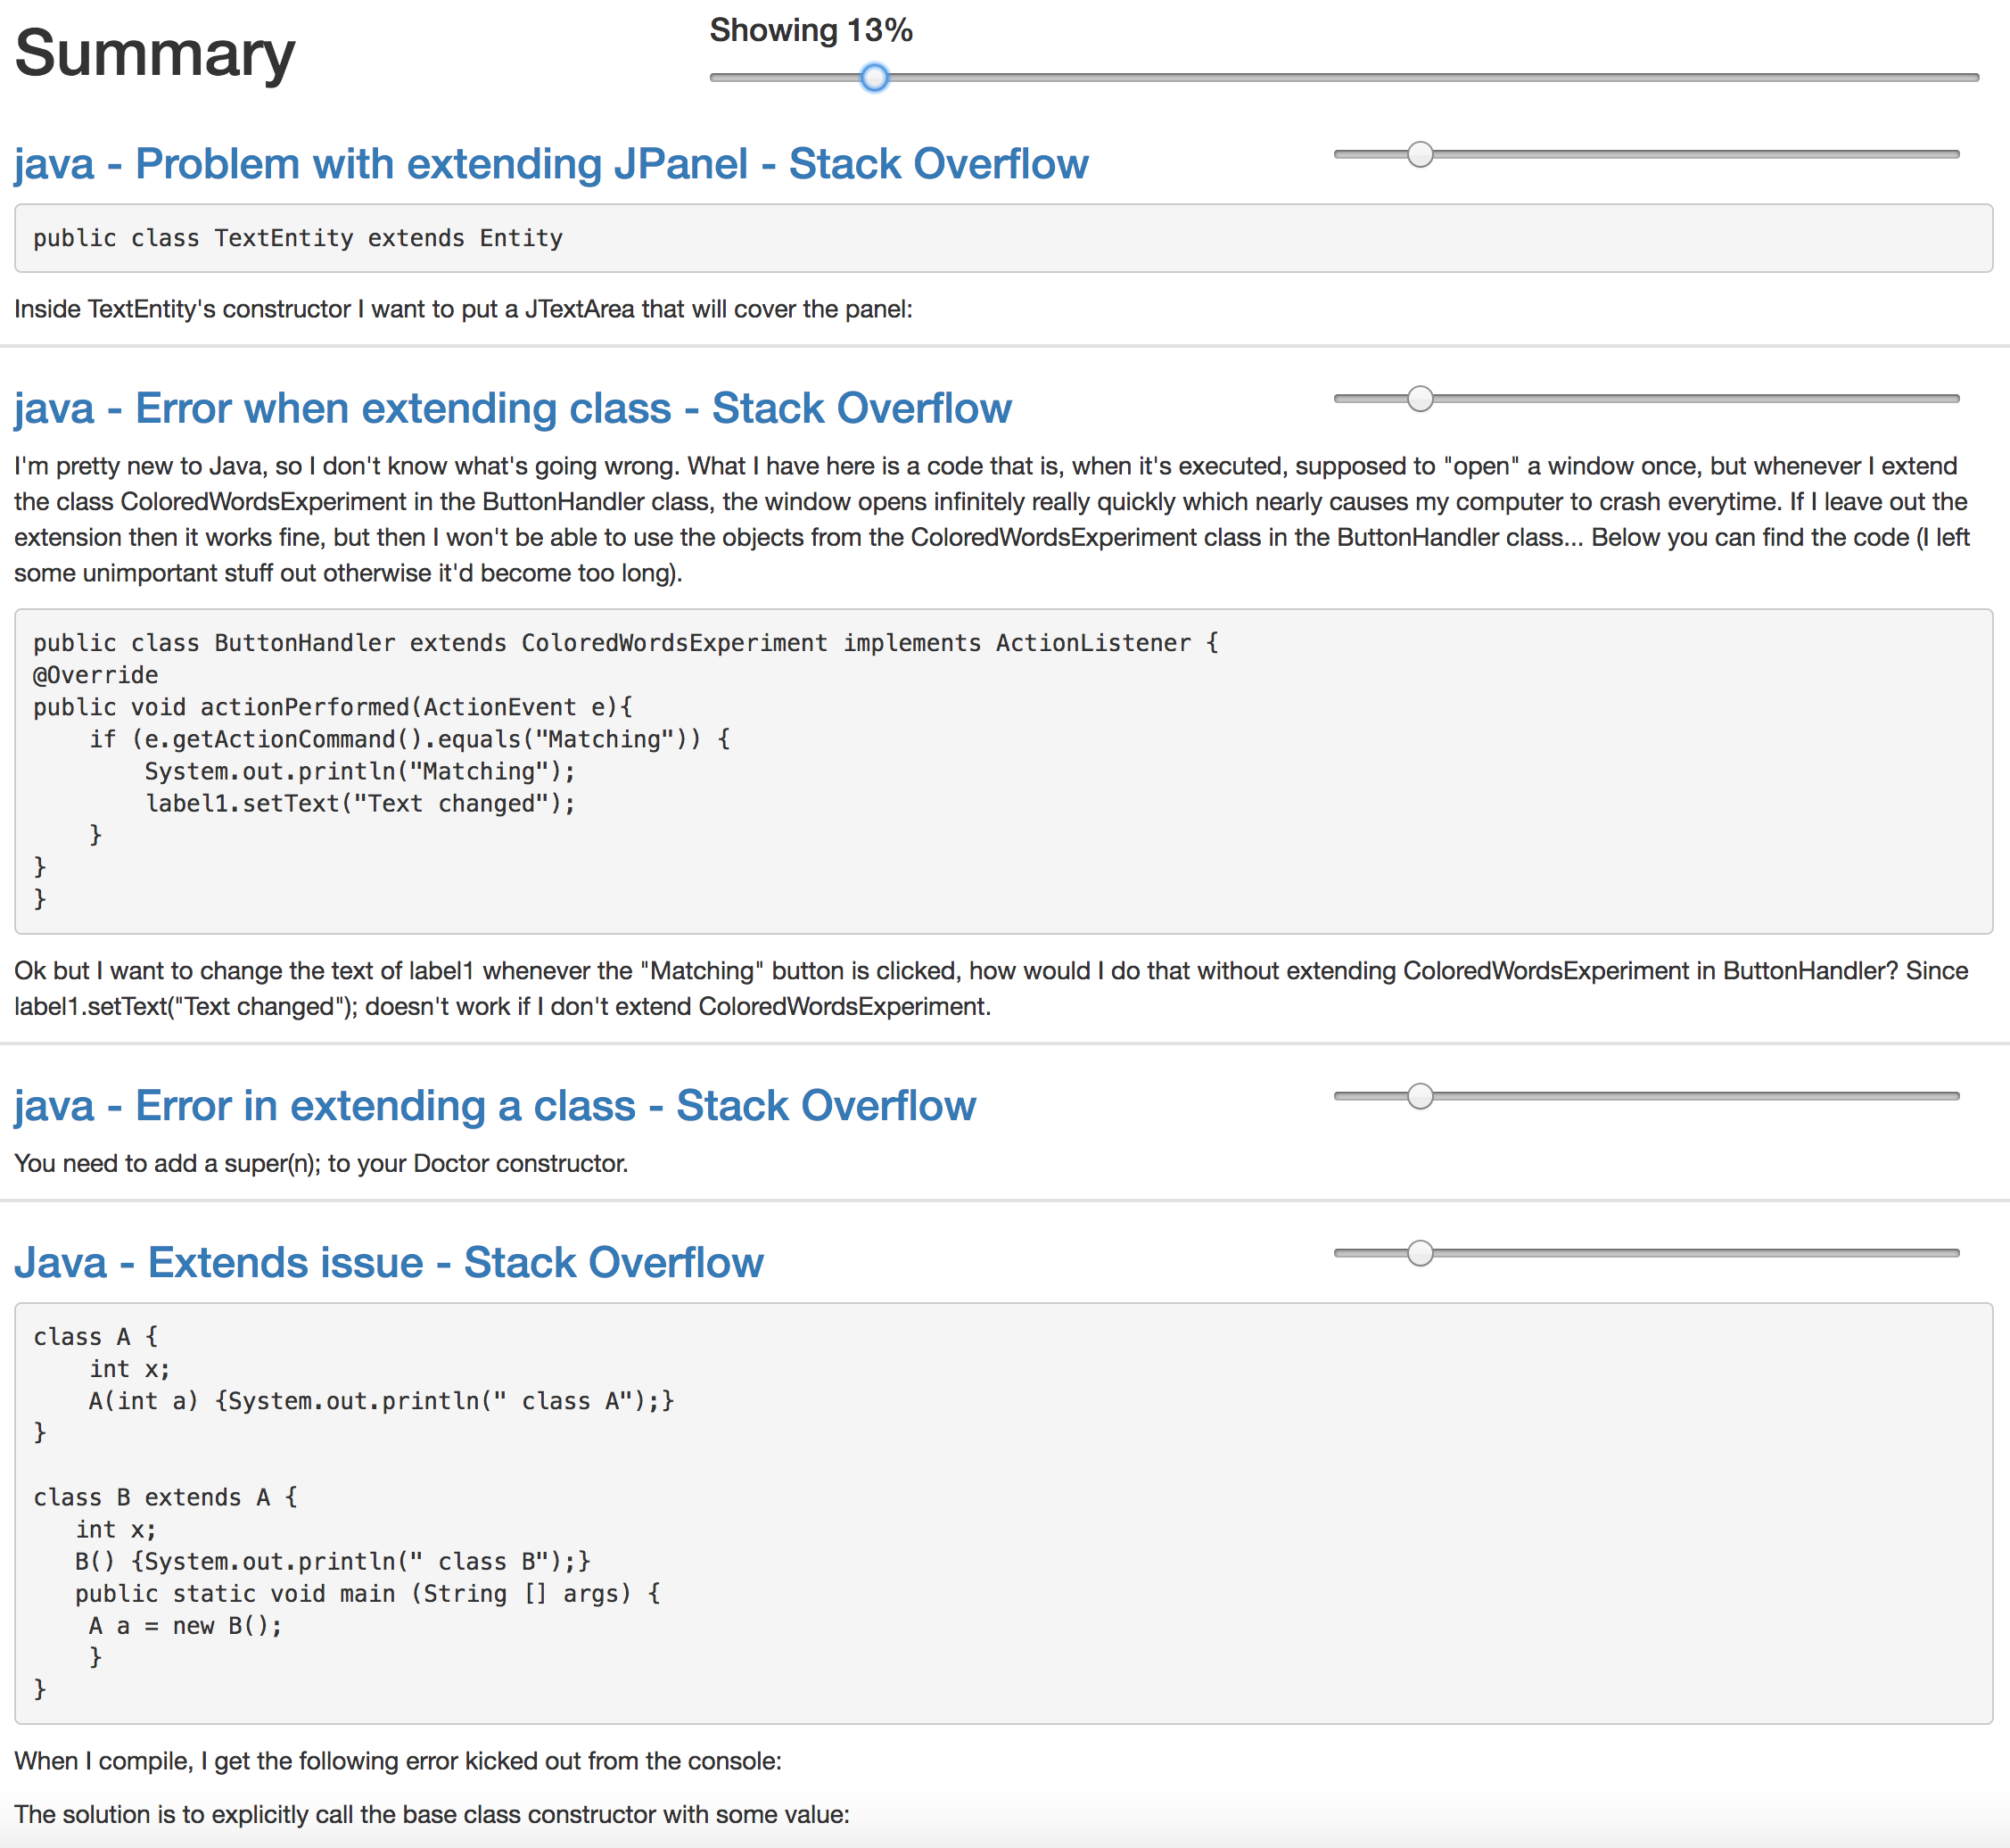
\includegraphics[scale=0.3]{Figures/SummaryExample}
\caption{Generated Summary}
\label{fig:chromeExtensionSummaryScreenshot}
\end{figure}
